\documentclass[../main.tex]{subfiles}

\begin{document}
Caustic is a transactional programming language for building race-free distributed systems. It
allows programmers to write applications as if they were single-threaded, but distribute them
arbitrarily without error.

In Section 1, we motivate the design of Caustic through a discussion of race conditions. In Section
2, we discuss the runtime and the various optimizations that allow it to efficiently and
transactionally execute programs. In Section 3, we extend the functionality of the runtime in a
robust, statically-typed Scala DSL called the standard library. In Section 4, we address
the syntactic limitations of the standard library by introducing the Caustic programming language
and its associated compiler.

% Race Conditions.
\section{Race Conditions}
\textbf{Race conditions} occur whenever the order in which concurrent programs are executed affects
their outcome. For example, suppose there exist two programs $A$ and $B$ that each increment a
shared counter $x$. Formally, each program reads the current value of $x$ and then writes $x + 1$.
If $B$ reads \emph{after} $A$ writes, then $B$ reads $x + 1$ and writes $x + 2$. However, if $B$
reads \emph{before} $A$ writes but after $A$ reads, then both $A$ and $B$ will read $x$ and write
$x + 1$. This is an example of a race condition, because the value of $x$ after both
$A$ and $B$ have \emph{completed} depends on the order in which $A$ and $B$ are \emph{executed}.
Race conditions may seem relatively benign, but they can have catastrophic consequences in practical
systems. Suppose the value of $x$ corresponded to your bank balance. What if your bank determined
your balance differently depending on the order in which deposits are made?

Before introducing mechanisms to deal with race conditions, we must first define the necessary and
sufficient criteria that any such mechanism must satisfy. Race conditions are a relatively
well-studied problem in database literature, and we may draw upon known results from the field to
define four properties of race-free programs.~\cite{transactions} We will hereafter refer to
any system that satisfies these properties as \textbf{transactional}.

\begin{itemize}
  \item \textbf{Atomic}: Programs never partially complete.
  \item \textbf{Consistent}: Programs see the effect of all completed programs.
  \item \textbf{Isolated}: Programs cannot see the effect of executing programs.
  \item \textbf{Durable}: The effects of completed programs are permanently visible.
\end{itemize}

  % Transactional Databases.
  \subsection{Transactional Databases}
  We begin our discussion of transactional systems with the same databases that we used to formalize
  their definition. Over the past few decades, transactional databases have made incredible advances
  in performance and scalability. While they provide the necessary guarantees on which correct
  distributed systems can be built, their query languages are not suitable for general-purpose
  programming for the following reasons.

  First, the absence of a standard query language tightly couples a database to the programs that
  are run on it. Relational databases, like MySQL and PostgreSQL, claim to implement the same SQL
  specification, but only support incompatible subsets of its functionality. Some NoSQL
  databases, like Cassandra and Aerospike, attempt to mimic SQL, but most implement their own
  bespoke interfaces. Stark differences between query languages makes it all but impossible to
  design general-purpose algorithms.

  Second, these query languages are lacking in functionality and programmability. Query languages
  are usually designed to access and modify data, but not to perform intermediate computation. For
  this reason, fundamental abstractions, like objects and variables, that programmers have come to
  rely on are glaringly absent in most query languages. Christopher Date, one of the fathers of
  relational databases, criticized SQL for its ambiguous and often unintuitive syntax.~\cite{sql}
  NoSQL databases are far worse, because they scale well only by shedding functionality.

  % Pessimistic Concurrency.
  \subsection{Pessimistic Concurrency}
  Another way to deal with race conditions is pessimistic concurrency, or \textbf{locking}.
  Before a program accesses or modifies shared data, it first declares its intentions to other
  programs by acquiring a lock that it subsequently releases when it is finished with the data.
  Locks are trivially transactional because they require programs to have exclusive ownership before
  performing any operations on shared data. However, locking introduces new problems.

  First, concurrent acquisition of multiple locks can cause a \textbf{deadlock} that prevents the
  system from making progress. For example, if program $A$ acquires lock $x$ and then attempts to
  acquire lock $y$ while program $B$ acquires $y$ and then attempts to acquire $x$, then neither $A$
  nor $B$ can make progress because each is waiting for the other to release their lock. This
  problem is typically mitigated by imposing a total order on lock acquisition; for any two locks
  $x$ and $y$, $x$ will always be acquired before $y$ or $y$ will always be acquired before $x$.
  Programs must be carefully constructed so that all locks are acquired in the universal order.

  Second, faulty programs may never release their locks. For example, if program $A$ acquires lock
  $x$ and subsequently fails, then no other program can ever acquire $x$. This problem is typically
  mitigated by using \textbf{leases}.~\cite{leases} A lease is a lock that is automatically released
  after a certain amount of time. Programs must be carefully constructed so that they complete their
  operations on shared data within the lease duration or refresh the lease before it expires.

  Third, locking is expensive. Locks must be acquired regardless of whether or not there actually
  are concurrent operations on shared data, because programs cannot know if there are or will be
  other programs that want or will want to simultaneously use the data. This significantly degrades
  performance in situations where contention between programs is low.

  Fourth, locking cannot protect against programmer error. Programmers may omit or incorrectly use a
  lock and thereby introduce race conditions into their program. Locks cannot guarantee that they
  will be used correctly, and, therefore, cannot guarantee that race conditions will be exhaustively
  eliminated from a program.

  % Optimistic Concurrency.
  \subsection{Optimistic Concurrency}
  A final alternative is optimisitic concurrency. Optimistic concurrency allows multiple programs to
  simultaneously access, but not modify, shared data without acquiring locks. Each program locally
  buffers any modifications that it makes and attempts to atomically apply them when it completes
  \emph{conditioned on the data that it accessed remaining unchanged}. If any data was modified, the
  program retries. This conditional update, known as a multi-word compare-and-swap, is known to be
  transactional and is widely used in a number of software transactional memory systems~\cite{stm}
  including Sinfonia~\cite{sinfonia} and Caustic. We will hereafter refer to this operation as
  \textbf{cas} and its arguments as a \textbf{transaction}.

  Optimistic concurrency requires a mechanism to detect that data has changed. The approach taken in
  Caustic and in similar systems is known as multi-version concurrency control. Data is uniquely
  identified by a \textbf{key} that is associated with a \textbf{revision}, or versioned value,
  whose version is incremented each time that its value is changed. We say that revisions $A$ and
  $B$ for a key \textbf{conflict} if the version of $A$ is less than $B$. Note that conflict is an
  asymmetric relation; if $A$ conflicts with $B$, then $B$ does not conflict with $A$.

  Optimistic concurrency assumes that contention between programs will be low, because frequent
  retries can significantly degrade performance. It also assumes the existence of an underlying
  key-value store, hereafter referred to as a \textbf{volume}, that supports \textbf{get} and
  \textbf{cas} which non-transactionally accesses and transactionally modifies data in the manner
  described above. We will provide a distributed, fault-tolerant implementation of a volume in
  Beaker. For now, we will assume that such an implementation exists.

% Runtime.
\section{Runtime}
A na\"ive implementation of optimistic concurrency would get each key whenever its value is needed
by a program. This approach performs well when volumes are located in memory, but does not scale
when they are on disk or across networks. Instead, a scalable implementation of optimistic
concurrency would get each key whenever its value is needed or \emph{will be needed} by a program.
This is the approach taken in the runtime.

\begin{figure}[htb]
  \caption{Concurrent Increment Program.}
  \centering
  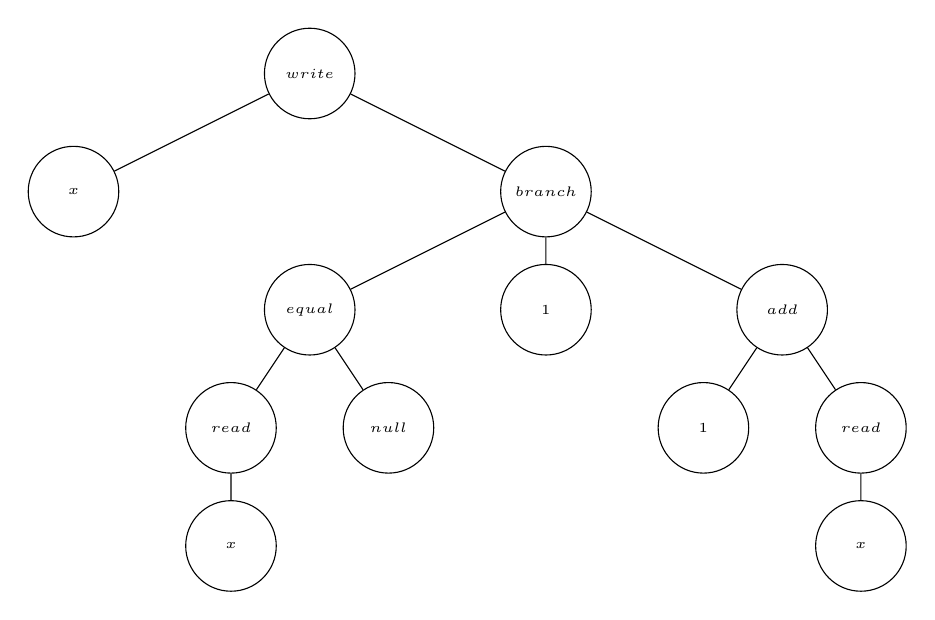
\begin{tikzpicture}[
    level/.style={sibling distance=60mm/#1},
    every node/.append style={draw, minimum height=1.15cm, align=center, font=\tiny}
  ]
    \node [circle, draw] (a) {$write$}
      child { node [circle, draw] (b) {$x$} }
      child { node [circle, draw] (e) {$branch$}
        child { node [circle, draw] (f) {$equal$}
          child { node [circle, draw] (g) {$read$}
            child { node [circle, draw] (h) {$x$} }
          }
          child { node [circle, draw] (i) {$null$} }
        }
        child { node [circle, draw] (j) {$1$} }
        child { node [circle, draw] (c) {$add$}
          child { node [circle, draw] (d) {$1$} }
          child { node [circle, draw] (k) {$read$}
            child { node [circle, draw] (l) {$x$} }
          }
        }
      };
  \end{tikzpicture}
  \label{figure:increment}
\end{figure}

The \textbf{runtime} is a virtual machine that dynamically translates \textbf{programs} into
transactions. A program is an abstract-syntax tree that is composed of \textbf{literals} and
\textbf{expressions}. A literal is a scalar value of type $flag$, $real$, $text$, or $null$ which
correspond to $bool$, $double$, $string$, and $null$ respectively in most C-style languages. An
expression is a function that transforms literal arguments into a literal result. For example,
Figure~\ref{figure:increment} is a program that increments a counter. Expressions may be chained
together arbitrarily to form complex programs. Table~\ref{table:expressions} enumerates the various
expressions that are natively supported by the runtime.

\begin{table}[ht]
  \caption{Instruction Set}
  \centering
  \begin{tabular}{l | l}
  \hline\hline
    Expression & Description                                                                      \\
    \hline
    add(x, y)                & Sum of $x$ and $y$.                                                \\
    both(x, y)               & Bitwise AND of $x$ and $y$.                                        \\
    branch(c, p, f)          & Executes $p$ if $c$ is true, or $f$ otherwise.                     \\
    cons(a, b)               & Executes $a$ and then $b$.                                         \\
    contains(x, y)           & Returns whether or not $x$ contains $y$.                           \\
    cos(x)                   & Cosine of $x$.                                                     \\
    div(x, y)                & Quotient of $x$ and $y$.                                           \\
    either(x, y)             & Bitwise OR of $x$ and $y$.                                         \\
    equal(x, y)              & Returns whether $x$ and $y$ are equal.                             \\
    floor(x)                 & Floor of $x$.                                                      \\
    indexOf(x, y)            & Returns the index of the first occurrence of $y$ in $x$.           \\
    length(x)                & Returns the number of characters in $x$.                           \\
    less(x, y)               & Returns whether $x$ is strictly less than $y$.                     \\
    load(n)                  & Loads the value of the variable $n$.                               \\
    log(x)                   & Natural log of $x$.                                                \\
    matches(x, y)            & Returns whether or not $x$ matches the regex pattern $y$.          \\
    mod(x, y)                & Remainder of $x$ divided by $y$.                                   \\
    mul(x, y)                & Product of $x$ and $y$.                                            \\
    negate(x)                & Bitwise negation of $x$.                                           \\
    pow(x, y)                & Returns $x$ raised to the power $y$.                               \\
    prefetch(k, s)           & Reads keys at $k/i$ for $i$ in $[0, s)$.                           \\
    read(k)                  & Reads the value of the key $k$.                                    \\
    repeat(c, b)             & Repeatedly executes $b$ while $c$ is true.                         \\
    rollback(r)              & Discards all writes and returns $r$.                               \\
    sin(x)                   & Sine of $x$.                                                       \\
    slice(x, l, h)           & Returns the substring of $x$ between $[l, h)$.                     \\
    store(n, v)              & Stores the value $v$ for the variable $n$.                         \\
    sub(x, y)                & Difference of $x$ and $y$.                                         \\
    write(k, v)              & Writes the value $v$ for the key $k$.                              \\
  \end{tabular}
  \label{table:expressions}
\end{table}

  % Execution.
  \subsection{Execution}
  The runtime uses iterative partial evaluation to gradually reduce programs into a
  single literal result according to the following procedure.

  \begin{enumerate}
    \item \textbf{Fetch}: Get all keys that are read or written anywhere in the program that have
          not been fetched before, and add the returned revisions to a local \textbf{snapshot}.
    \item \textbf{Evaluate}: Recursively replace all expressions with literal arguments with their
          corresponding literal result. For example,

          \[
          \begin{gathered}
          add(real(1), sub(real(0), real(2))) \rightarrow real(-1)
          \end{gathered}
          \]

          The result of all writes is saved to a local \textbf{buffer} and the result of all reads
          is the latest value of the key in the local buffer or snapshot. This ensures that reads
          will see the effect of all previous writes within the program.
    \item \textbf{Repeat}: Loop until the program is reduced to a single literal. Because all
          expressions with literal arguments return a literal result, all programs will eventually
          reduce to a single literal.
    \item \textbf{Commit}: Cas all keys in the local buffer conditioned on all revisions in
          the local snapshot. The transactional guarantees of cas imply that program execution is
          \textbf{serializable}. Serializability means that concurrent execution has the
          same effect as some sequential execution, and, therefore, that program execution will be
          robust against race conditions.
  \end{enumerate}

  % Optimizations.
  \subsection{Optimizations}
  First, execution is tail-recursive. This allows programs to be composed of arbitrarily many
  nested expressions without overflowing the stack frame during execution. It also allows the Scala
  compiler to aggressively optimize execution into a tight loop.

  Second, the runtime batches I/O. Reads are performed simultaneously whenever possible and writes
  are buffered and simultaneously committed. By batching I/O, the runtime performs a minimal number
  of operations on the database. This has significant performance implications, because I/O overhead
  is overwhelmingly the bottleneck by many orders of magnitude in most programs.~\cite{io}

  Third, the runtime performs constant folding. Expressions with literal arguments are automatically
  simplified. This significantly reduces the size of programs and thereby improves the performance
  of the runtime.

  % Performance.
  \subsection{Performance}
  \begin{figure}[ht]
    \caption{Runtime Performance}
    \label{figure:performance}
    \centering
    \begin{tikzpicture}
      \begin{axis}[
      width=.38\textwidth,
      xlabel={Program Size},
      ylabel={Latency (ms)},
      ]
        \addplot[only marks, mark = *]
        table {data/runtime-latency.dat};
        \addplot[thick, red]
        table[y={create col/linear regression={y=latency}}] {data/runtime-latency.dat};
      \end{axis}
    \end{tikzpicture}
    ~
    \begin{tikzpicture}
      \begin{axis}[
      width=.38\textwidth,
      xlabel={Threads},
      ylabel={Throughput (ops/sec)},
      scaled y ticks=false,
      cycle list name=mark list,
      legend cell align={left},
      legend style={at={(1.03,1)}, anchor=north west, draw=black, fill=white, align=left},
      ]
        \addplot
        table[y index=1] {data/runtime-throughput.dat};
        \addlegendentry{R 1.0\% W 0.0\%};
        \addplot
        table[y index=2] {data/runtime-throughput.dat};
        \addlegendentry{R 0.0\% W 0.1\%};
        \addplot
        table[y index=3] {data/runtime-throughput.dat};
        \addlegendentry{R 0.0\% W 0.5\%};
        \addplot
        table[y index=4] {data/runtime-throughput.dat};
        \addlegendentry{R 0.0\% W 1.0\%};
        \addplot
        table[y index=5] {data/runtime-throughput.dat};
        \addlegendentry{R 1.0\% W 1.0\%};
        \addplot
        table[y index=6] {data/runtime-throughput.dat};
        \addlegendentry{R 0.0\% W 2.0\%};
      \end{axis}
    \end{tikzpicture}
  \end{figure}

  In Figure~\ref{figure:performance}, we examine execution latency and throughput. Benchmarks were
  conducted on a t2.2xlarge instance with 32GB of RAM and 8 CPUs. We first see that latency
  grows linearly with program size. In other words, \emph{each additional expression has a constant
  overhead}. We then graph throughput under a variety of workloads. Each workload is composed of the
  specified number of threads simultaneously executing a series of programs that each read and write
  the specified percentages of the key-space uniformly at random. Note that the larger the
  percentage of writes and the greater the number of threads, the more likely that cas
  will fail and the more significant the reduction in throughput will be. We see that in read-only
  workloads, throughput scales linearly with the number of threads. As the percentage of writes and
  the number of threads increases, throughput falls considerably but still scales linearly with the
  number of threads.

% Standard Library.
\section{Standard Library}
The runtime provides native support for an extremely limited subset of the operations that
programmers typically rely on to write applications. The standard library supplements the
functionality of the runtime by exposing a robust Scala DSL complete with static types, records,
collections, math, and control flow.

  % Typing.
  \subsection{Typing}
  The runtime natively supports just four dynamic types: $flag$, $real$, $text$, and $null$.
  Dynamic versus static typing is a religious debate among programmers. Advocates of dynamic
  typing often mistakenly believe that type inference and coercive subtyping cannot be provided by
  a static type system. In fact, they can. Because static type systems are able to
  detect type inaccuracies at compile-time, they allow programmers to write more concise and
  correct code.~\cite{typing} The standard library provides rich static types and features
  aggressive type inference and subtype polymorphism.

  The standard library supports four \textbf{primitive} types. In ascending order of precedence,
  they are \textbf{boolean}, \textbf{int}, \textbf{double}, and \textbf{string}. A \texbf{value}
  represents a value of primitive type. There are two kinds of values. A \textbf{constant} is an
  immutable value, and a \textbf{variable} is a mutable value. Variables may be stored locally in
  memory or remotely in a volume.

  \begin{lstlisting}[style=Scala]
    // Creates an integer local variable named x.
    val x = Variable.Local[Int]("x")
    // Creates a floating point remote variable named y.
    val y = Variable.Remote[Double]("y")
    // Assigns y to the sum of x and y.
    y := x + y
    // Assigns x to the product of x and 4.
    x *= 4
    // Does not compile, because y is not an integer.
    x := y
    // Does compile, because floor(y) is an integer.
    x := floor(y)
  \end{lstlisting}

  % Records.
  \subsection{Records}
  In addition to these primitive types, the standard library also supports \textbf{references} to
  user-defined records. References use \href{https://github.com/milessabin/shapeless}{Shapeless} to
  materialize compiler macros that permit the fields of a record to be statically manipulated and
  iterated. A current limitation is that records cannot be self-referential; a record cannot have a
  field of its own type.

  \begin{lstlisting}[style=Scala]
    // An example type declaration.
    case class Bar(
      a: String,
    )

    case class Foo(
      b: Int,
      c: Reference[Bar],
      d: Bar
    )

    // Constructs a remote reference to a Foo.
    val x = Reference[Foo](Variable.Remote("x"))
    // Returns the value of the field b.
    x.get(@<'b>@)
    // Does not compile, because z is not a field of Foo.
    x.get(@<'z>@)
    // Serializes x to a JSON string.
    x.asJson
    // Deletes all fields of x and all references.
    x.delete(recursive = true)
    // Constructs a local reference to a Foo.
    val y = Reference[Foo](Variable.Local("y"))
    // Copies x to y.
    y := x
  \end{lstlisting}

  % Collections.
  \subsection{Collections}
  The runtime has no native support for collections of key-value pairs. The standard library
  provides implementations of three fundamental data structures: \textbf{list}, \textbf{set},
  and \textbf{map}. These collections are mutable and statically-typed. Collections take care of the
  messy details of mapping structured data onto a flat namespace and feature prefetched iteration.
  A current limitation is that collections may only contain primitive types.

  \begin{lstlisting}[style=Scala]
    // Constructs a map from string to boolean.
    val x = Map[String, Boolean](Variable.Remote("y"))
    // Puts an entry in the map.
    x += "foo" -> true
    // Serializes x to a JSON string.
    x.asJson
    // Constructs a list of integers.
    val x = List[Int](Variable.Local("x"))
    // Increments each element in the list.
    x foreach { case (i, v) => x.set(i, v + 1) }
  \end{lstlisting}

  % Math.
  \subsection{Math}
  The runtime natively supports just nine mathematical operations: $add$, $sub$, $mul$, $div$,
  $pow$, $log$, $floor$, $sin$, and $cos$. However, these primitive operations are sufficient to
  derive the entire Scala \href{https://www.scala-lang.org/api/2.12.1/scala/math/index.html}{math}
  library using various mathematical identities and approximations. The $div$, $log$, $sin$, and
  $cos$ functions can actually be implemented in terms of the other primitive operations; however,
  native support for them was included in the runtime to improve performance. The standard library
  provides implementations for all functions enumerated in Table~\ref{table:math}.

  \begin{lstlisting}[style=Scala]
    // Returns the Taylor approximation of inverse sine.
    asin(Pi / 2)
    // Defines the sigmoid function.
    def sigmoid(x: Value[Double]) = exp(x) / (exp(x) + 1)
  \end{lstlisting}


  \begin{table}[ht]
    \caption{Math}
    \centering
    \begin{tabular}{l | l}
    \hline\hline
      Function & Description                                                                      \\
      \hline
      abs(x)                   & Absolute value of $x$.                                           \\
      acos(x)                  & Cosine inverse of $x$.                                           \\
      acot(x)                  & Cotangent inverse of $x$.                                        \\
      acsc(x)                  & Consecant inverse of $x$.                                        \\
      asec(x)                  & Secant inverse of $x$.                                           \\
      asin(x)                  & Sine inverse of $x$.                                             \\
      atan(x)                  & Tangent inverse of $x$.                                          \\
      cbrt(x)                  & Cube root of $x$.                                                \\
      ceil(x)                  & Smallest integer greater than or equal to $x$.                   \\
      cos(x)                   & Cosine of $x$.                                                   \\
      cosh(x)                  & Hyperbolic cosine of $x$.                                        \\
      cot(x)                   & Cotangent of $x$.                                                \\
      coth(x)                  & Hyperbolic cotangent of $x$.                                     \\
      csc(x)                   & Cosecant of $x$.                                                 \\
      csch(x)                  & Hyperbolic cosecant of $x$.                                      \\
      exp(x)                   & Exponential of $x$.                                              \\
      expm1(x)                 & Equivalent to $e^x - 1$.                                         \\
      floor(x)                 & Largest integer less than or equal to $x$.                       \\
      hypot(x, y)              & Hypotenuse of the triangle with base $x$ and height $y$.         \\
      log(x)                   & Natural logarithm of $x$.                                        \\
      log10(x)                 & Log base 10 of $x$.                                              \\
      log1p(x)                 & Equivalent to $\log (x + 1)$.                                    \\
      pow(x, y)                & Power of $x$ to the $y$.                                         \\
      random()                 & Uniformly random number on [0, 1).                               \\
      rint(x)                  & Closest integer to $x$, rounding to the nearest even number.     \\
      round(x)                 & Closest integer to $x$, rounding up.                             \\
      round(x, y)              & Closest multiple of $y$ to $x$.                                  \\
      sec(x)                   & Secant of $x$.                                                   \\
      sech(x)                  & Hyperbolic secant of $x$.                                        \\
      signum(x)                & Sign of $x$.                                                     \\
      sin(x)                   & Sine of $x$.                                                     \\
      sinh(x)                  & Hyperbolic sine of $x$.                                          \\
      sqrt(x)                  & Square root of $x$.                                              \\
      tan(x)                   & Tangent of $x$.                                                  \\
      tanh(x)                  & Hyperbolic tangent of $x$.                                       \\
    \end{tabular}
    \label{table:math}
  \end{table}

  % Control Flow.
  \subsection{Control Flow}
  The runtime natively supports control flow operations like $branch$, $cons$, and $repeat$.
  However, these operations are syntactically challenging to express. The standard library
  uses structural types to provide support for \textbf{if}, \textbf{while}, \textbf{return},
  \textbf{assert}, and \textbf{rollback}.

  \begin{lstlisting}[style=Scala]
    // If statements.
    If (x < 3) {
      x += 3
    }

    // If/Else statements
    If (y < x) {
      y += 1
    } Else {
      x += 1
    }

    // Ternary operator.
    val z = If (y === x) { y - 1 } Else { y + 1 }

    // While loops.
    While (x <> y) {
      x *= 2
    }
  \end{lstlisting}

% Compiler.
\section{Compiler}
The standard library provides additional functionality that is absent in the runtime to make it
easier to construct programs. However, it does not address the syntactic challenges of expressing
programs. At times the standard library is forced to use unintuitive operators like $:=$ and $<>$
and verbose declarations like $Variable.Remote(``x")$, because of the limitations of implementing a
language within a language.

The \textbf{compiler}, Causticc, translates code written in the Caustic programming language
into operations on the standard library. Caustic features aggressive type inference, static typing,
and a concise grammar.

  % Implementation.
  \subsection{Implementation}
  We use ANTLR~\cite{antlr} to generate a predicated LL(*) parser from an ANTLR grammar and then
  walk the resulting parse-tree to generate code. Most statements in Caustic have direct equivalents
  in the standard library. For the most part, the compiler acts as a kind of intelligent
  find-and-replace. However, there are certain aspects of the compiler that are non-trivial.

  First, the compiler performs type inference. It is able statically verify types and method
  signatures by maintaining a lexically-scoped \textbf{universe} of the various variables, records,
  and functions that have been defined. Because the type system is relatively simplistic, static
  types almost never need to be specified. The combination of a static type system and aggressive
  type inference allows programs to be both type-safe and concise.

  Second, the compiler is directly integrated \href{https://www.pantsbuild.org/}{Pants}. Pants is an
  open-source, cross-language build system. Integration into Pants means that Caustic programs are
  interoperable with a variety of existing languages and tooling.

  Third, the compiler provides a \href{https://macromates.com/}{TextMate} bundle that implements
  syntax highlighting and code completion for most text editors and IDEs to make it easier for
  programmers to use the language.

  % Programmability.
  \subsection{Programmability}
  Programmability is impossible to measure, because there is no metric by which two languages can be
  objectively compared. We will present implementations of various algorithms in Caustic and in
  other languages, but, instead of comparing them with an imprecise measure of programmability like
  lines of code or cyclomatic complexity, we will reserve all judgement and leave it to the reader
  to verify for themselves that Caustic is indeed easier to use.

  Consider the following example of a distributed counter written in Caustic. A similar
  implementation of a distributed, backend-agnostic counter is provided by
  \href{https://git.io/vxS6u}{Akka}.

  \begin{lstlisting}[style=Caustic]
    module caustic.example

    /**
     * A distributed counter.
     */
    service Counter {

      /**
       * Increments the total and returns its current value.
       *
       * @param x Reference to total.
       * @return Current value.
       */
      def increment(x: Int&): Int = {
        if (x != null) x += 1 else x = 1
        x
      }

    }
  \end{lstlisting}

  Consider the following example of a distributed file system in Caustic.

  \begin{lstlisting}[style=Caustic]
    module caustic.example

    /**
     * A file.
     *
     * @param contents File contents.
     */
    struct File {
      contents: String
    }

    /**
     * A distributed file system.
     */
    service FileSystem {

      /**
       * Returns the contents of the specified path.
       *
       * @param path File path.
       * @return Current contents.
       */
      def read(path: File&): String = path.contents

      /**
       * Returns whether or not the file exists.
       *
       * @param path File path.
       * @return Whether or not the file exists.
       */
      def exists(path: File&): String = path.contents != null

      /**
       * Updates the contents of the specified path.
       *
       * @param path File path.
       * @param contents File contents.
       */
      def write(path: File&, contents: String): Unit =
        path.contents = contents

      /**
       * Deletes the specified path.
       *
       * @param path File path.
       */
      def delete(path: File&): Unit = del path

    }
  \end{lstlisting}

  Consider the following example of a distributed message queue written in Caustic. A similar
  implementation of a distributed queue is provided by \href{https://git.io/vpOT}{Curator}.

  \begin{lstlisting}[style=Caustic]
    module caustic.example

    /**
     * A distributed message queue.
     */
    service Queue {

      /**
       * Adds the message to the end of the queue.
       *
       * @param queue Queue.
       * @param message Message.
       */
      def push(queue: List[String]&, message: String): Unit =
        queue.set(queue.size, message)

      /**
       * Returns the message at the front of the queue.
       *
       * @param queue Queue.
       * @return Head.
       */
      def peek(queue: List[String]&): String = queue.get(0)

      /**
       * Removes and returns the message at the front of the queue.
       *
       * @param queue Queue.
       * @return Head.
       */
      def pop(queue: List[String]&): String = {
        var head = peek(queue)
        queue.set(0, null)
        head
      }

      /**
       * Returns the number of messages in the queue.
       *
       * @param queue Queue.
       * @return Length.
       */
      def size(queue: List[String]&): Int = queue.size

    }
  \end{lstlisting}

  Consider the following example of a distributed lock service written in Caustic. A similar
  implementation of a distributed read-write lock is provided by
  \href{https://git.io/vpOTL}{Curator} and \href{https://git.io/vpOTq}{Sherlock}.

  \begin{lstlisting}[style=Caustic]
    module caustic.example

    /**
     * A read-write lock.
     *
     * @param readers Number of readers.
     * @param writers Number of writers.
     */
    struct Lock {
      readers: Int,
      writers: Int
    }

    /**
     * An access permit.
     *
     * @param lock Underlying lock.
     * @param forRead Read access.
     * @param forWrite Write access.
     */
    struct Permit {
      lock: Lock&,
      forRead: Boolean,
      forWrite: Boolean
    }

    /**
     * A distributed lock service.
     */
    service LockService {

      /**
       * Attempts to acquire exclusive access to the lock.
       *
       * @param lock Lock.
       * @return Read-write permit.
       */
      def exclusive(lock: Lock&): Permit = {
        if (lock.writers > 0 || lock.readers > 0) {
          Permit(lock, false, false)
        } else {
          lock.writers += 1
          Permit(lock, false, true)
        }
      }

      /**
       * Attempts to acquire shared access to the lock.
       *
       * @param lock Lock.
       * @return Read-only permit.
       */
      def shared(lock: Lock&): Permit = {
        if (lock.writers > 0) {
          Permit(lock, false, false)
        } else {
          lock.readers += 1
          Permit(lock, true, false)
        }
      }

      /**
       * Revoke the permit's access.
       *
       * @param permit Permit.
       */
      def release(permit: Permit): Unit = {
        if (permit.forRead) {
          permit.lock.readers -= 1
        } elif (permit.forWrite) {
          permit.lock.writers -= 1
        }
      }
    
    }
  \end{lstlisting}

% Conclusion.
\section{Conclusion}
Concurrency is difficult, but it does not need to be. Caustic allows programmers to build concurrent
systems as if they were they were not. It provides a highly programmable alternative to traditional
approaches for dealing with race conditions. We have shown that it is possible to build a robust,
transactional programming language over any volume that supports just two operations. In Beaker, we
will see that these operations can be efficiently implemented.

\end{document}